\documentclass[11pt]{article}

% ==== Paquetes ====
\usepackage[utf8]{inputenc}
\usepackage[spanish]{babel}
\usepackage{amsmath, amssymb, amsfonts, siunitx}
\usepackage{graphicx}
\usepackage{float}
\usepackage{listings} % Para código
\usepackage{xcolor}
\usepackage{hyperref}
\usepackage{caption}
\usepackage{subcaption}
\usepackage{geometry}
\usepackage{tikz}

\geometry{margin=2.5cm}

% ==== Configuración de listings (para código) ====
\lstset{
  basicstyle=\ttfamily\small,
  numbers=left,
  numberstyle=\tiny,
  stepnumber=1,
  numbersep=5pt,
  backgroundcolor=\color{gray!10},
  frame=single,
  tabsize=2,
  breaklines=true,
  showstringspaces=false,
  keywordstyle=\color{blue},
  commentstyle=\color{green!50!black},
  stringstyle=\color{red!70!black}
}

% ==== Datos de la tarea ====
\title{IEE3584 - Comunicaciones inalámbricas \\
Tarea 2}
\author{Nicolás Seguel}
\date{Agosto 2025}

\begin{document}
\maketitle

% ==== Ejemplo de respuesta con texto y fórmulas ====
\section*{Problema 4}

A partir del modelo de señal recibida para el Caso Ia dada por

\[
\tilde{r}(t) = \lambda_p \breve{h} \tilde{s} (t) + \tilde{n}(t),
\]

y de la arquitectura del receptor con VGA y ecualizador para este caso, analice la razón señal a ruido por símbolo de:

\begin{enumerate}
    \item la señal antes del VGA,
    \item entre el VGA y el filtro adaptado,
    \item después del muestreador del filtro adaptado y antes del ecualizador, y
    \item después del ecualizador.
    \item Concluya a partir de su análisis que \(\lambda_p\) no altera la razón señal a ruido en todo el recorrido de la señal en el receptor, y que por lo tanto es posible simplificar el modelo de señal \(\lambda_p = 1\), o bien absorbiendo \(\lambda_p\) bajo la densidad espectral de potencia del ruido \(N_0\), como elemento integrante de la razón señal a ruido.
\end{enumerate}

\subsection*{Solución}

\subitem{1. La señal antes del VGA}

La potencia de la señal recibida antes del VGA es:

\begin{equation*}
    P_{r} = E\left\{|\tilde{r}(t)|^2\right\} = \lambda_p^2 \breve{h}^2 E_s
\end{equation*}

Ahora bien la potencia del ruido es:

\begin{equation*}
    P_{n} = E\left\{|\tilde{n}(t)|^2\right\} = N_0 B
\end{equation*}

Por lo tanto, la razón señal a ruido antes del VGA es:

\begin{equation*}
    \text{SNR} = \frac{P_{r}}{P_{n}} = \frac{\lambda_p^2 \breve{h}^2 E_s}{N_0 B}
\end{equation*}

\subitem{2. Entre el VGA y el filtro adaptado}

La señal después del VGA es:

\begin{equation*}
    \tilde{r}_{\text{VGA}}(t) = G \tilde{r}(t) = G (\lambda_p \breve{h} \tilde{s}(t) + \tilde{n}(t)) = G \lambda_p \breve{h} \tilde{s}(t) + G \tilde{n}(t)
\end{equation*}

Por lo tanto, la razón señal a ruido entre el VGA y el filtro adaptado es:

\[
SNR_{\text{VGA}} = \frac{G^2 \lambda_p^2 \breve{h}^2 E_s}{G^2 N_0 B} = \frac{\lambda_p^2 \breve{h}^2 E_s}{N_0 B}
\]

que es identica a la razón señal a ruido antes del VGA.

\subitem{3. Después del muestreador del filtro adaptado y antes del ecualizador}

La señal después del filtro adaptado y el muestreador es:

\begin{equation*}
    \tilde{r}_{\text{FA}}[k] = \int \tilde{r}_{\text{VGA}}(t) h^*(t - kT) dt = G \lambda_p \breve{h} \tilde{s}[k] + \tilde{n}_{\text{FA}}[k]
\end{equation*}

donde \(\tilde{n}_{\text{FA}}[k]\) es el ruido después del filtro adaptado y el muestreador, cuya potencia es:

\begin{equation*}
    P_{n, \text{FA}} = E\left\{|\tilde{n}_{\text{FA}}[k]|^2\right\} = N_0
\end{equation*}

Por lo tanto, la razón señal a ruido después del muestreador del filtro adaptado y antes del ecualizador es:

\begin{equation*}
    SNR_{\text{FA}} = \frac{G^2 \lambda_p^2 \breve{h}^2 E_s}{N_0} = \frac{\lambda_p^2 \breve{h}^2 E_s}{N_0}
\end{equation*}

\subitem{4. Después del ecualizador}

La señal después del ecualizador es:

\begin{equation*}
    \tilde{r}_{\text{EQ}}[k] = \tilde{r}_{\text{FA}}[k] * c[k] = G \lambda_p \breve{h} \tilde{s}[k] * c[k] + \tilde{n}_{\text{FA}}[k] * c[k]
\end{equation*}

donde \(c[k]\) es la respuesta al impulso del ecualizador. La potencia del ruido después del ecualizador es:

\begin{equation*}
    P_{n, \text{EQ}} = E\left\{|\tilde{n}_{\text{FA}}[k] * c[k]|^2\right\} = N_0 \sum |c[k]|^2
\end{equation*}

Por lo tanto, la razón señal a ruido después del ecualizador es:

\begin{equation*}
    SNR_{\text{EQ}} = \frac{G^2 \lambda_p^2 \breve{h}^2 E_s \sum |c[k]|^2}{N_0 \sum |c[k]|^2} = \frac{\lambda_p^2 \breve{h}^2 E_s}{N_0}
\end{equation*}

\subitem{5. Conclusión}

En todos los puntos analizados del receptor, la razón señal a ruido es:

\begin{equation*}
    SNR = \frac{\lambda_p^2 \breve{h}^2 E_s}{N_0 B} \quad \text{o} \quad SNR = \frac{\lambda_p^2 \breve{h}^2 E_s}{N_0}
\end{equation*}

lo que demuestra que los elementos del receptor no alteran la razón señal a ruido. Además se observa que \(\lambda_p\) aparece como un factor multiplicativo en el numerador, por lo que puede ser absorbido en la densidad espectral de potencia del ruido \(N_0\) o simplificado a 1 sin alterar la razón señal a ruido en todo el recorrido de la señal en el receptor.

\section*{Problema 5}

A partir del modelo de desvaneciemiento local del Caso 1a, dado por:

\begin{align}
    \breve{h} &= \sum_{n=1}^{L_c} h_n e^{j \varphi_n} \\
    & = \sum_{n=1}^{L_c} h_n \left( \cos(\varphi_n) + j \sin(\varphi_n) \right) \\
    & = h_I + j h_Q
\end{align}

y de algunos supuestos sobre el número de trayectorias Lc, las magnitudes \(h_n\) y fases $\varphi_n$, la aplicación del Teorema del Límite Central permite establecer que:

\begin{equation*}
    h_I, h_Q \sim \mathcal{N}(0, \sigma^2)
\end{equation*}

Muestre que:

\begin{enumerate}
    \item \(\nu = E\left\{h_I\right\} = E\left\{h_Q\right\} = 0\)
    \item \(\sigma^2 = E\left\{h_I^2\right\} = E\left\{h_Q^2\right\} = \frac{1}{2}\)
    \item Muestre además que \(E\left\{h_I h_Q\right\} = 0\), lo que permite concluir que \(\breve{h} \sim N_c(0,1)\).
\end{enumerate}

\subsection*{Solución}

\subsubitem{1. \(\nu = E\left\{h_I\right\} = E\left\{h_Q\right\} = 0\)}

Dado que \(h_I\) y \(h_Q\) son con densidad de probabilidad \(\mathcal{N}(0, \sigma^2)\), la media es cero para ambas variables:

\[
E\left\{h_I\right\} = \sum_{i=1}^{L_c} E\left\{h_n \cos(\varphi_n)\right\} = \sum_{i=1}^{L_c} E\left\{h_n\right\} E\left\{\cos(\varphi_n)\right\} = 0
\]

donde la esperanza de \(\cos(\varphi_n)\) es cero debido a la distribución uniforme de \(\varphi_n\) en \([0, 2\pi)\). De manera similar, se puede demostrar que \(E\left\{h_Q\right\} = 0\).

\subsubitem{2. \(\sigma^2 = E\left\{h_I^2\right\} = E\left\{h_Q^2\right\} = \frac{1}{2}\)}

La varianza de \(h_I\) es:

\[
E\left\{h_I^2\right\} = \sum_{i_1 = 1}^{L_c} \sum_{i_2 = 1}^{L_c} E\left\{h_{i_1} h_{i_2} \cos(\varphi_{i_1}) \cos(\varphi_{i_2})\right\}
\]

Dado que las fases \(\varphi_n\) son independientes y uniformemente distribuidas, los términos cruzados donde \(i_1 \neq i_2\) tienen esperanza cero. Por lo tanto, solo los términos donde \(i_1 = i_2\) contribuyen a la suma:

\[
E\left\{h_I^2\right\} = \sum_{i=1}^{L_c} E\left\{h_i^2\right\} E\left\{\cos^2(\varphi_i)\right\} = E\left\{\sum_{i = 1}^{L_c} h_i^2 \right\}  \cdot \frac{1}{2} = \frac{1}{2}
\]

donde se ha utilizado que \(E\left\{\cos^2(\varphi_i)\right\} = \frac{1}{2}\) debido a la distribución uniforme de \(\varphi_i\) en \([0, 2\pi)\), y que \(E\left\{\sum_{i = 1}^{L_c} h_i^2 \right\} = 1\) por la normalización de las potencias de las trayectorias. De manera similar, se puede demostrar que \(E\left\{h_Q^2\right\} = \frac{1}{2}\).

\subsubitem{3. Muestre además que \(E\left\{h_I h_Q\right\} = 0\).}

La covarianza entre \(h_I\) y \(h_Q\) es:

\[
E\left\{h_I h_Q\right\} = E\left\{\left(\sum_{i=1}^{L_c} h_i \cos(\varphi_i)\right) \left(\sum_{j=1}^{L_c} h_j \sin(\varphi_j)\right)\right\}
\]

Dado que las fases \(\varphi_n\) son independientes y uniformemente distribuidas, los términos cruzados donde \(i \neq j\) tienen esperanza cero. Por lo tanto, solo los términos donde \(i = j\) contribuyen a la suma:

\[
E\left\{h_I h_Q\right\} = \sum_{i=1}^{L_c} E\left\{h_i^2 \cos(\varphi_i) \sin(\varphi_i)\right\} = E\left\{\sum_{i=1}^{L_c} h_i^2 \right\}  \cdot E\left\{\cos(\varphi_i) \sin(\varphi_i)\right\} = 0
\]

donde se ha utilizado que \(E\left\{\cos(\varphi_i) \sin(\varphi_i)\right\} = 0\) debido a la distribución uniforme de \(\varphi_i\) en \([0, 2\pi)\).

Por lo tanto, \(h_I\) y \(h_Q\) son variables aleatorias independientes con media cero y varianza \(\frac{1}{2}\), lo que implica que \(\breve{h} = h_I + j h_Q\) es una variable aleatoria compleja normal con media cero y varianza 1, es decir, \(\breve{h} \sim N_c(0,1)\).

\section*{Problema 6}

Considere la variable aleatoria Rayleigh r que resulta de las variables
aleatorias Normales \(h_I\) y \(h_Q\), ambas con media cero y varianza \(\sigma^2\), mediante la transformación \(r = \sqrt{h_I^2 + h_Q^2}\). La función de distribución de probabilidad de r esta dada por:

\begin{equation*}
    p(r) = \frac{r}{\sigma^2} e^{-\frac{r^2}{2\sigma^2}}, \quad r \geq 0
\end{equation*}

Calcule:

\begin{enumerate}
    \item La función de acumulación de probabilidad de r, \(F_r(R) = P(r \leq R)\).
    \item La media de la distribución de Rayleigh, \(E\{r\}\).
    \item La varianza de la distribución de Rayleigh, \(E\left\{r^2\right\} - E\{r\}^2\).
    \item El valor más probable de la distribución. \(\text{máx}_r \left\{p(r)\right\}\).
    \item La mediana de la distribución, es decir, \(R\) tal que \(F_r(R) = \frac{1}{2}\).
\end{enumerate}

\subsection*{Solución}

\subitem{1. La función de acumulación de probabilidad de r, \(F_r(R) = P(r \leq R)\).}

La función de acumulación de probabilidad \(F_r(R)\) se obtiene integrando la función de densidad de probabilidad \(p(r)\) desde 0 hasta \(R\):

\begin{align*}
    F_r(R) &= \int_0^R p(r) dr \\
    &= \int_0^R \frac{r}{\sigma^2} e^{-\frac{r^2}{2\sigma^2}} dr \\
    &= 1 - e^{-\frac{R^2}{2\sigma^2}}
\end{align*}

\subitem{2. La media de la distribución de Rayleigh, \(E\{r\}\).}

La media de la distribución de Rayleigh se calcula como:

\begin{align*}
    E\{r\} &= \int_0^\infty r p(r) dr \\
    &= \int_0^\infty r \frac{r}{\sigma^2} e^{-\frac{r^2}{2\sigma^2}} dr \\
    &= \frac{1}{\sigma^2} \int_0^\infty r^2 e^{-\frac{r^2}{2\sigma^2}} dr \\
    &= \sigma \sqrt{\frac{\pi}{2}}
\end{align*}

\subitem{3. La varianza de la distribución de Rayleigh, \(E\left\{r^2\right\} - E\{r\}^2\).}

La varianza de la distribución de Rayleigh se calcula como:

\begin{align*}
    E\left\{r^2\right\} &= \int_0^\infty r^2 p(r) dr \\
    &= \int_0^\infty r^2 \frac{r}{\sigma^2} e^{-\frac{r^2}{2\sigma^2}} dr \\
    &= \frac{1}{\sigma^2} \int_0^\infty r^3 e^{-\frac{r^2}{2\sigma^2}} dr \\
    &= 2\sigma^2
\end{align*}

Por lo tanto, la varianza es:

\begin{align*}
    \text{Var}(r) &= E\left\{r^2\right\} - E\{r\}^2 \\
    &= 2\sigma^2 - \left(\sigma \sqrt{\frac{\pi}{2}}\right)^2 \\
    &= \sigma^2 \left(2 - \frac{\pi}{2}\right)
\end{align*}

\subitem{4. El valor más probable de la distribución. \(\text{máx}_r \left\{p(r)\right\}\).}

El valor más probable de la distribución se encuentra en la función de densidad de probabilidad \(p(r)\) evaluada en \(\sigma\):

\begin{align*}
    \text{máx}_r \left\{p(r)\right\} &= p(\sigma) \\
    &= \frac{\sigma}{\sigma^2} e^{-\frac{\sigma^2}{2\sigma^2}} \\
    &= \frac{1}{\sigma} e^{-\frac{1}{2}} \\
    &= \frac{1}{\sigma \sqrt{e}}
\end{align*}

\subitem{5. La mediana de la distribución, es decir, \(R\) tal que \(F_r(R) = \frac{1}{2}\).}

La mediana de la distribución se encuentra resolviendo la ecuación \(F_r(R) = \frac{1}{2}\):

\begin{align*}
    F_r(R) &= \frac{1}{2} \\
    1 - e^{-\frac{R^2}{2\sigma^2}} &= \frac{1}{2} \\
    e^{-\frac{R^2}{2\sigma^2}} &= \frac{1}{2} \\
    -\frac{R^2}{2\sigma^2} &= \ln\left(\frac{1}{2}\right) \\
    R^2 &= -2\sigma^2 \ln\left(\frac{1}{2}\right) \\
    R &= \sigma \sqrt{2 \ln(2)}
\end{align*}

\section*{Problema 7}

Verifique computacionalmente cada uno de los resultados del Problema 6. Para ello, genere una cantidad enorme (\(\geq 10^5\)) de números aleatorios gaussianos para \(h_I\) y \(h_Q\) con \(\sigma_h = 1\), y calcule numéricamente el estadístico que corresponda (partes b, c, d y e). Indique en cada caso el valor obtenido. Incluya además un histograma (normalizado) de la distribución de la fase y magnitud de \(h_I + j h_Q\), y sobreponga la curva teórica para comparación. Utilice el histograma para generar y graficar la función de acumulación de probabilidad (parte a).

\subsection*{Solución}

\begin{figure}[H]
    \centering
    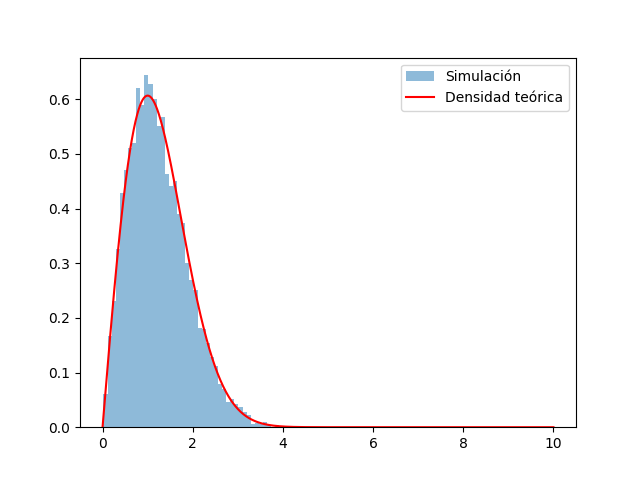
\includegraphics[width=0.8\textwidth]{Figure_1.png}
    \caption{Histograma de la magnitud \(r\) con la curva teórica superpuesta.}
    \label{fig:magnitud}
\end{figure}

Los resultados obtenidos son:

\begin{itemize}
    \item Media \(E\{r\}\): 1.2422 (Teórico: 1.2533)
    \item Varianza \(\text{Var}(r)\): 0.4296 (Teórico: 0.4292)
    \item Valor más probable \(\text{máx}_r \left\{p(r)\right\}\): 1 (Teórico: 1)
    \item Mediana \(R\) tal que \(F_r(R) = \frac{1}{2}\): 1.1514 (Teórico: 1.1774)
\end{itemize}

\lstinputlisting[language=Python, caption=Código en Python para verificar los resultados del Problema 6.]{p7.py}

\end{document}
